\documentclass[11pt, a4paper, oneside, twocolumn, dvipdfmx]{jsarticle}
\usepackage{url}
\usepackage{graphicx}
\usepackage{geometry}
\geometry{top=1cm,  bottom=2cm, left=1.5cm, right=1.5cm}
\pagestyle{empty}
\usepackage{amsmath}
\usepackage{tikz}
\usetikzlibrary{intersections,calc,arrows.meta}
\setlength{\intextsep}{10pt}
\setlength{\textfloatsep}{10pt}

\newcommand{\simname}{SimSym}
\newcommand{\simnamealt}{Simulation with Symbols}

\title{物理学の学習のためのプログラマブルな
\\シミュレータと環境の提案}

\author{東京工業大学 情報理工学院 数理・計算科学系\\18B04657 木内康介\\指導教員 増原英彦教授}

\date{}

\begin{document}
\maketitle

\section{はじめに} \label{intro}
高等学校における物理学の授業において、実験は重要である。Holubova~\cite{holubova_2019}は、実験室での作業は理論的な概念を検証する最も重要な方法であり、生徒は実験を通してどのような現象が起きるかを確認することができると述べている。% TODO: 具体化

しかし実際は、生徒全員が実験を経験しているわけではない。力学分野において最も基本的な「運動の法則」に関する実験の実施経験は、2014年の調査時点で60\%にしか満たない~\cite{2015KJ00010038066}。
理由としては、実験用の装置の準備や測定が難しいことや、実験を行うのに時間を要することが考えられる。

そこで実験の代替として近年利用されているのが、物理実験のシミュレーションである。シミュレーションを用いることで、実験と同様の学習効果を得ることができる~\cite{ajredini_real_2014}。

しかし、実際に生徒が解く問題の解答過程と既存のシミュレータでは、確認できる情報の間にギャップがある。高等学校で扱う物理の問題では図~\ref{symbol_based}のように物理量として文字を利用した方程式の計算を要求される。一方、例えばPhET~\cite{perkins_phet_2006} は、図~\ref{numeral_based}のように速度や質量、位置を数値のみで表現していて、可視化された運動がどのような方程式や導出過程を表現しているものなのか確認することができない。

\begin{figure}[b]
% 静止している質量 $m$ の物体に大きさ $F$ の力をかけ続ける。 $t$ 秒後の速度の大きさを求めよ。
\begin{align}
  \left\{
  \begin{aligned}
    ma &= F & (1)\\
    v &= at & (2)
  \end{aligned}
  \right. \nonumber
\end{align}
(1)より、$a = \dfrac{F}{m}$ \quad (2)に代入して、$v = \dfrac{F}{m}t$
\centering
% 答え: $\dfrac{F}{m}t$
\caption{方程式の計算例} \label{symbol_based}
\end{figure}

\begin{figure}[thb]
  \centering
  \includegraphics*[width=0.9\linewidth]{figure/PhET_example.png}
  \caption{PhET のシミュレーション例} \label{numeral_based}
  \end{figure}

そこで本研究では、物体の運動を方程式で定義できるシミュレータである \simname~(\simnamealt) を提案する。\simname では、シミュレーションを実行すると、定義した方程式に基づいて数値計算がなされ、物体の運動が可視化される。
% これにより、ユーザが導出した方程式がどのような運動と対応するか簡単に確認することができる。
さらに、ユーザは $(\text{位置}) + (\text{速度})$ のように異なる次元の間の和や差を含む方程式は定義することができない。そのため、単純な計算ミスなどを検出することができる。

なお、\simname は大部分が未実装である。そのため、\ref{sec2}節の内容は基本的にはアイデアであるが、\ref{sec3}節に記す方針で実装が可能であると考えている。

\section{\simname} \label{sec2}

\simname は、ブラウザ上で実行できるシミュレータである。ユーザは以下の操作を行う:

\begin{enumerate}
\item 物体の作成: 物体の名前を入力し物体作成ボタンを押すと、その物体と描画に最低限必要なフィールド(x座標・y座標)が生成される。質量や速度などのフィールドは自由に追加することができる。
\item 方程式の作成: ユーザが定数・変数を自由に追加し、方程式を定義する。この際、定数と変数には初期値と次元(長さ、質量等)を設定する必要がある。なお、時刻を表す変数 $t$ は用意されている。その後、追加した定数・変数を使って方程式を定義する。長さとキログラムの和など、次元が一致していない方程式は警告され、定義できない。
\item 物体と方程式の紐付け: 方程式を物体のフィールドにドラッグすると、そのフィールドに方程式を紐付け、フィールドの値を方程式に数値を代入した結果にすることができる。方程式とフィールドの次元が一致していない場合、紐付けることはできない。
\item シミュレーションの実行: シミュレーションを再生すると、時刻 $t$ が変化しながら各方程式が計算され、方程式に基づいて物体が運動する。
\end{enumerate}

以下では具体例を見ていく。図~\ref{simsym_fig1}は、\simname 上で斜方投射を表現した例である。この例ではy座標に紐付けている方程式が $v_{0y}t - \frac{gt^2}{2}$ となっているため、シミュレーションを再生すると図~\ref{correct}のような軌道を描く。ここで、速度の次元を持つ $gt$ という方程式はy座標に紐付けることができない。また、$(\text{位置}) - (\text{速度})$ という形になっている $v_{0y}t - gt$ という方程式を作成しようとすると、次元が一致していないため警告され、定義できない。

\begin{figure}[htb]
  \centering
  \includegraphics*[width=0.9\linewidth]{work/slide_img4-crop.pdf}
  \caption{\simname 上で斜方投射を表現した例} \label{simsym_fig1}
\end{figure}

\begin{figure}[htb]
\centering
% \begin{minipage}{0.4\linewidth}
\begin{minipage}{0.8\linewidth}
\centering
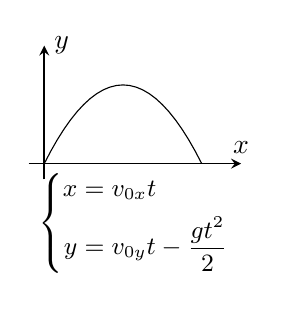
\begin{tikzpicture}
\draw[->,>=stealth,semithick](-0.2,0)--(2.5,0)node[above]{$x$}node[anchor=north east]{$\small{\left\{ \begin{aligned} x &= v_{0x}t \\ y &= v_{0y}t-\frac{gt^2}{2} \end{aligned} \right.}$};
\draw[->,>=stealth,semithick](0,-0.2)--(0,1.5)node[right]{$y$};
\draw[domain=0:2]plot(\x,{-1 * pow(\x-1, 2) + 1});
\end{tikzpicture}
\caption{斜方投射の軌道} \label{correct}
\end{minipage}
% \begin{minipage}{0.4\linewidth}
% \centering
% \begin{tikzpicture}
% \draw[->,>=stealth,semithick](-0.2,0)--(2.5,0)node[above]{$x$}node[anchor=north east]{$\small{\left\{ \begin{aligned} x &= v_{0x}t \\ y &= v_{0y}t+\frac{gt^2}{2} \end{aligned} \right.}$};
% \draw[->,>=stealth,semithick](0,-0.2)--(0,2.5)node[right]{$y$};
% \draw[domain=0:2]plot(\x, {(pow(\x+1, 2) - 1) / 4});
% \end{tikzpicture}
% \caption{誤った軌道} \label{wrong}
% \end{minipage}
\end{figure}

\section{実装の方針} \label{sec3}
実装は、フロントエンドに lively.next\footnote{\url{https://lively-next.org}} を、方程式の定義や数値代入に SymPy~\cite{meurer_sympy_2017} を用い、JavaScriptで行う。

\subsection*{lively.next}
lively.next は、GUIアプリケーションを作成・実行するためのWebプログラミング環境である。これを用いることで、ブラウザ上で簡単にGUIアプリケーションが実行できる。ユーザが物体や定数、方程式を定義するインターフェースとシミュレーションを表示する画面を lively.next で作成する。

\subsection*{SymPy}
SymPy は、記号計算のための Python ライブラリである。lively.next に入力された定数や方程式を SymPy の方程式に変換し、数値計算を行い、その結果を lively.next で表示する。Python ライブラリであるが、Pyodide~\footnote{\url{https://pyodide.org/en/stable/}} を用いることで WebAssembly に変換し、ブラウザ上で実行させる。

% \subsection{Pyodide}
% Pyodide は、WebAssembly で実装された CPython 処理系である。ブラウザ上で Python 並びにいくつかのパッケージを実行することができる。これを用いて、lively.next から SymPy を呼び出して計算することをブラウザ上だけで完結させることができる。

\section{まとめと課題}
本研究では方程式で物体の動きを定義できるシミュレータ \simname を提案した。\simname を用いることで、生徒は自身が導出した文字式がどのような動きと対応するか確認することができる。

今後の課題は、方程式から動きを想像する力が付き、物理学に対するより直感的・本質的な理解が得られることを確認するための \simname の教育効果の評価である。評価手法として、Hake~\cite{hake_1998}が導入した normalized gain を用いた実験を検討する。

\bibliographystyle{junsrt}
\bibliography{thesis}

\end{document}